\section{Overview of \name}
\begin{figure}[t]
\centering
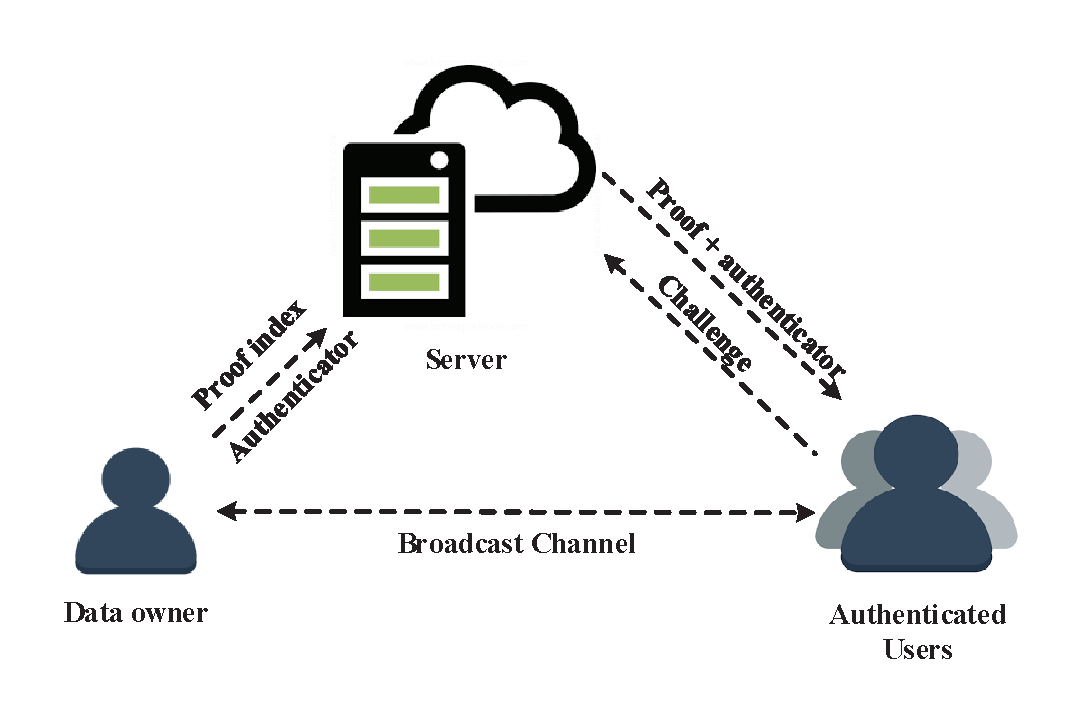
\includegraphics[width=2.5 in]{model}
\DeclareGraphicsExtensions.
\caption{System architecture of \name on the three-party model.}
\label{fig:model}
\end{figure}

In this section, we present an overview of our \name scheme. The major notations used in this paper are shown in Table~\ref{tab:notations}.

\begin{table}[h]
  \begin{center}
  \caption{Notations}
  \label{tab:notations}
  %\begin{threeparttable}
  \begin{tabular}{|c|c|}
    \hline
    Notation      &Meaning  \\
    \hline
    \hline
    $\mathcal{W}$ & keyword set \\
    \hline
    $|W|$         & \blue{size of the keyword set}   \\
    \hline
    $w_i$         & keyword, where $i \in \{1, \cdots, |W|\}$\\
    \hline
    $\mathcal{D}$ & plaintext of the document set \\
    \hline
    $D_{w_i}$     & plaintext of a document set containing $w_i$\\
    \hline
    $\mathcal{C}$ & ciphertext of the document set \\
    \hline
    $C_{w_i}$     & ciphertext of a document set containing $w_i$ \\
    \hline
    $f$           & plaintext of a document  \\
    \hline
    $c$           & ciphertext of a document \\
    \hline
    $W_f$         & keyword set of document $f$\\
    \hline
    $\tau$        & the search token (challenge)\\
    \hline
    $\lambda$     & the proof index. \\
    \hline
    $\pi$         & the authenticator.\\
    \hline
  \end{tabular}\\
  \end{center}
\end{table}


\subsection{System architechture}
Fig.~\ref{fig:model} illustrates the system architecture of \name. It consists of three parties: \blue{{\em data owners}, who provide the encrypted proof index corresponding to their data and authenticators to cloud services}; the {\em untrusted server}, which provides storage and search services; \blue{a set of {\em authenticated users}, who challenge the cloud services for verification of search results retrieved from the SSE scheme.}



\subsection{System model}
We aim to develop a verifiable SSE scheme, i.e., \name, that allows the index used for search result verification to be separated from the one used for the SSE operations. Therefore, \name is decoupled from the existing SSE schemes. \blue{In particular, data owner will builds an encrypted index based on the Merkle Patricia Tree (MPT) and upload it to cloud services, which enables data users to verify the integrity of search results. Meanwhile, data owner will also upload a timestamp-chain based on the root of MPT to ensure data freshness across multiple users.}
\name is defined as follows.

\begin{definition}[\textbf{\name Scheme}]\label{def:name}
  {\itshape
      In a \name scheme, there are three parties, i.e., data owners, authenticated users and an untrusted server.  A data owner provides a proof index and an authenticator to the untrusted server such that it allows the server to provide a proof of the search result and authenticators for the authenticated users to ensure the integrity and freshness of the SSE search results. A \name scheme is a collection of seven polynomial-time algorithms, where
      \begin{itemize}
        \item \red{$KGen(1^k) \rightarrow \{K_1,K_2,K_3, (ssk, spk)\}$: is a probabilistic algorithm run by the data owner. It takes as input a security parameter, and outputs the secret keys $K_1,K_2,K_3$ and a random signing keypair $(ssk, spk)$.}
        \item \red{$Init(K_1,K_2,K_3, ssk, \mathcal{D}) \rightarrow \{\lambda,\pi\}$: is an algorithms run by the data owner which takes as input the symmetric keys $K_1,K_2,K_3$, the signing secret key $ssk$}, and the document set $\mathcal{D}$, and outputs the proof index $\lambda$ and the anthenticator $\pi$. The data owner stores the proof $\lambda$ locally and meanwhile sends $\lambda$ and $\pi$ to the server.
        \item \red{$PreUpdate(K_1,K_2,K_3, ssk, f) \rightarrow \{\tau_u, \pi\}$: is an algorithm run by the data owner. It takes as input the symmetric keys $K_1,K_2,K_3$, the signing secret key $ssk$}, and a file $f$ to be updated, and outputs the update tokens $\tau_u$ and the authenticator $\pi$. The data owner sends $\tau_u$ and $\pi$ to the server.
        \item $Update(\lambda, \tau_u) \rightarrow \{\lambda'\}$: is an algorithm run by the server. It takes as input the proof index $\lambda$ and the update tokens $\tau_u$, and outputs the new proof index $\lambda'$;
        \item $Challenge(K_1, w) \rightarrow \{\tau_{w}\}$: is a deterministic algorithm run by the user. It takes as input a symmetric key $K_1$ and a specific keyword $w$, and outputs a challenge $\tau_{w}$ corresponding to $w$. The user sends the challenge $\tau_{w}$ to the server.
        \item \blue{$Prove(\lambda, \tau_{w}, t_q) \rightarrow \{\rho,\pi^t_q, \pi_c\}$: is an algorithm run by the server. It takes as input the proof index $\lambda$, the challenge $\tau_{w}$, and the query time $t_q$, it outputs the proof $\rho$ and authenticators $\pi^t_q$,$\pi_c$. The server sends $\rho$ and authenticators $\pi^t_q$,$\pi_c$ to the requested user.}
        \item \red{$Verify(K_1,K_2,K_3, spk, C_w, \rho, \pi^t_q, \pi_c, \tau_{w}) \rightarrow \{b\}$: is an algorithm run by the data user which takes as input symmetric keys $K_1,K_2,K_3$, the public key $spk$, the SSE search result $C_w$, the proof $\rho$, authenticators $\pi^t_q, \pi_c$ and the challenge token $\tau_{w}$, it outputs a bit $b$ represent an $accept$ or $reject$ result. This algorithm consists of two sub-algorithms,  the Check algorithm and the Generate algorithm, which can be written as $Check(K_3, spk, \pi^t_q, \pi_c) \rightarrow \{b\}$ and $Generate(K_1,K_2,K_3,C_w,\rho,\tau_{w},\pi^t_q) \rightarrow \{b\}$.}
        %\item \blue{$Verify(K_1,K_2,K_3, C_w, \rho, \pi^t_q, \pi_c, \tau_{w}) \rightarrow \{b\}$: is an algorithm run by the data user which consists of two sub-algorithms. One is the Check algorithm $Check(K_3, \pi^t_q, \pi_c) \rightarrow \{b\}$, which takes as input the tuples $<K_3, \pi^t_q, \pi_c>$, and outputs a bit $b$. The other is the Generate algorithm $Generate(K_1,K_2,K_3,C_w,\rho,\tau_{w},\pi^t_q) \rightarrow \{b\}$, which takes as input the the symmetric keys $K_1,K_2,K_3$, the SSE search result $C_w$, the proof $\rho$, the challenge token $\tau_{w}$ and the authenticator $\pi^t_q$, and it outputs a bit $b$. Finally, the Verify algorithm outputs a bit $b$ represent an $accept$ or $reject$ result.}
      \end{itemize}
      }
\end{definition}
